\documentclass[11pt, oneside, a4paper]{book}

% ----------------------------------------------------------------------------
% Preamble
% ----------------------------------------------------------------------------

% Package to manage page layout
\usepackage[a4paper, top=25.4mm, bottom=25.4mm, right=25.4mm, left=40mm]{geometry}

% Line spacing: single=1 one-and-a-half=1.3 double=1.6
\linespread{1.3}

% Package to manage appendix
\usepackage[toc]{appendix}

% Package to insert empty lines between paragraphs
\usepackage[parfill]{parskip}

% Package to manage headers and footers
\usepackage{fancyhdr}

% define two header-footer styles
% 'normal' for most pages
\fancypagestyle{normal}{
\fancyhf{}
\fancyhead[L]{\slshape \leftmark} %chapter
\fancyhead[R]{\thepage} %footer
\renewcommand{\headrulewidth}{1pt}
}
% 'chapterstyle' for start of chapters (no chapter in header)
\fancypagestyle{chapterstyle}{
    \fancyhf{}
    \fancyhead[R]{\thepage}
    \renewcommand{\headrulewidth}{0pt}% Line at the header invisible
}

% Package to automatically change headerfooter style at start of chapters
\usepackage{etoolbox}
\patchcmd{\chapter}{\thispagestyle{plain}}{\thispagestyle{chapterstyle}}{}{}


% Package to get hyperrlinks
\usepackage{hyperref}

% Mathematics packages
\usepackage{amsmath}
\usepackage{amssymb}
\usepackage{mathtools}

% A package to include graphics files (jpg, png, eps, pdf etc...)
\usepackage{graphicx}

% A package that gives more control for bibliographies than the default
\usepackage[backend=biber,
			maxcitenames=2,
			maxbibnames=99,
			doi=false,
			url=false,
			bibstyle=apa,
			firstinits,
			uniquename=init,
			style=authoryear
            ]{biblatex}
\addbibresource{bibliography.bib}


% Package to add features for tables
\usepackage{multirow}
\usepackage{booktabs}
\setlength{\heavyrulewidth}{1.5pt}
\setlength{\abovetopsep}{4pt}

% Package to allow sub-figures
\usepackage{subcaption}


% A package to generate latin. You do not need this: I am just using it to get
% random text.
\usepackage{lipsum}

\usepackage{standalone}
\usepackage{tikz}
\usetikzlibrary{er,positioning, calc, patterns}
\usetikzlibrary{decorations.pathreplacing}
% ----------------------------------------------------------------------------
% The actual report
% ----------------------------------------------------------------------------

\begin{document}

\newgeometry{a4paper, top=25.4mm, bottom=25.4mm, right=25.4mm, left=25.4mm}
\begin{titlepage}
	\begin{center}
		\vspace*{1cm}
		\vspace{10pt}

		\hrule
		\vspace{10pt}
		\huge
		\textsc{Understanding responses to environments for the Prisoner's Dilemma:
		A meta analysis, multidimensional optimisation and machine learning approach}
		\vspace{15pt}
		\hrule
		
		\vspace{2cm}

		
\includegraphics[width=40mm]{cardiff_logo.jpg}
		\vspace{1cm}

		\LARGE
		Nikoleta E. Glynatsi
		
		\vspace{2cm}
		\large
		Submitted in partial fulfillment of\\ the requirements for the degree of\\[0.35em] Doctor of Philosophy. \\
		\vspace{1cm}
		May 2020

	\end{center}
\end{titlepage}
\restoregeometry

\frontmatter
\pagestyle{chapterstyle} %set header-footer style for front matter
\chapter{Executive Summary}

\lipsum[1-9]
\chapter{Acknowledgements}

First and foremost, I would like to express my greatest and utmost gratitude to
my tolerant and supportive supervisor, Dr Vincent Knight, whose guidance,
encouragement and jokes have been invaluable throughout my PhD. I am extremely
grateful for our long research meetings, our friendly chats that concluded with
me spoiling a movie/show for you, and our academic trips around the world.

I would also like to thank Dr Jonathan Gillard for his advice through parts of
this work and Dr Marc Harper for his input and commentary in the narrative on
the meta tournaments research.

On a more personal note, I would like to thank my family who have been a source
of great inspiration and motivation throughout life. They never questioned my
decisions and have supported me to the fullest. Except that time when my mother
disapproved of me travelling to New York alone.  I would like to express  my
sincere gratitude to my friends Nicki Verdeli, Kostas Soulanis and Chris
Athanasiou, for their continuous support and friendship throughout my years in
Cardiff. Their homemade meals, inspirational talks about not getting anxious and
competitive games of UNO have been vital in the completion of this PhD. 

I would also like to thank my colleagues Waleed Ali, Asyl Hawa, Geraint Palmer,
Chris Seaman, Lorenzo De Biase, Henry Wilde and Emily O'Riordan for their
company and endless coffee breaks. Finally, I would like to thank Mrs Joanna
Emery for making my academic journey in Cardiff University possible, and the
professional services staff of the School for Mathematics for their continuous
help the past four years with filling forms, booking rooms, resolving IT issues
and preparing coffee and biscuits.

\tableofcontents
\listoffigures
\listoftables
\chapter{Summary}

\lipsum[1-3]

\mainmatter
\pagestyle{normal} %set header-footer style rest of report


\chapter{Introduction}
% \input{chapters/chapter2.tex}
% \input{chapters/chapter3.tex}
% \input{chapters/chapter4.tex}



\addcontentsline{toc}{chapter}{References}
\printbibliography[title=References]

\begin{appendices}
% \chapter{Centrality measures distributions}

\section{Distributions for \(G\) and \(\bar{G}\)}

Betweeness and closeness centralities distributions for \(G\) and \(\bar{G}\).

\begin{figure}[!hbtp]
    \centering
    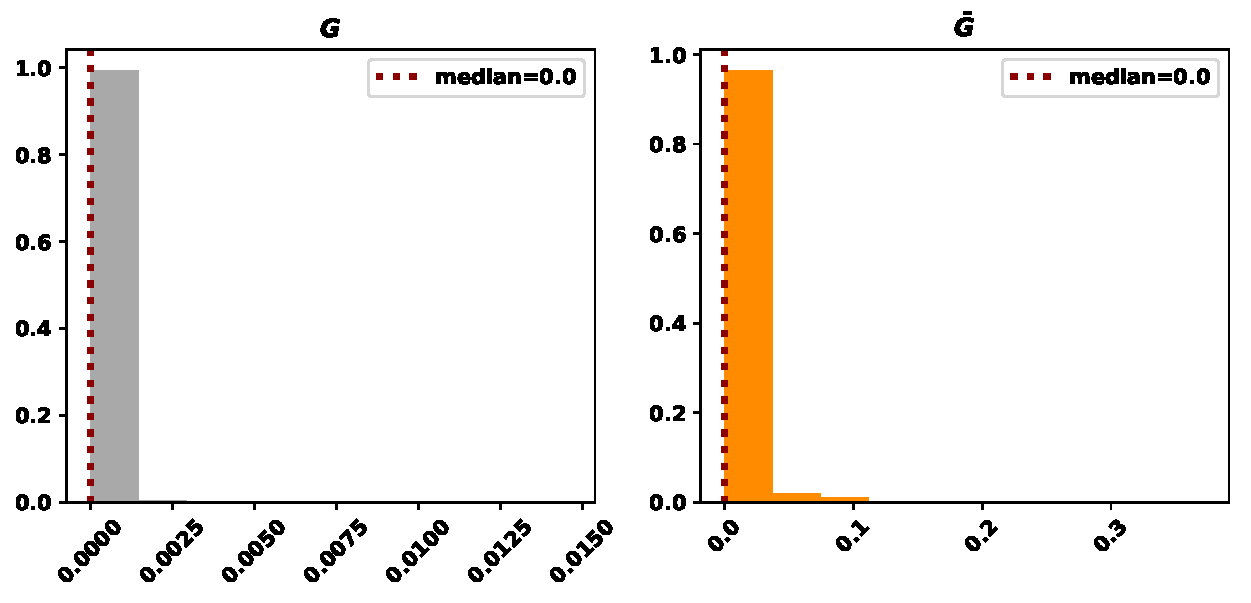
\includegraphics[width=.8\textwidth]{src/chapters/03/paper/bibliometric-study-of-the-prisoners-dilemma/assets/images/pd_betweeness_centralities.pdf}
    \caption{Distributions of betweenness centrality in \(G\) and \(\bar{G}\)}
    \label{fig:bc_distributions}
\end{figure}

\begin{figure}[!hbtp]
    \centering
    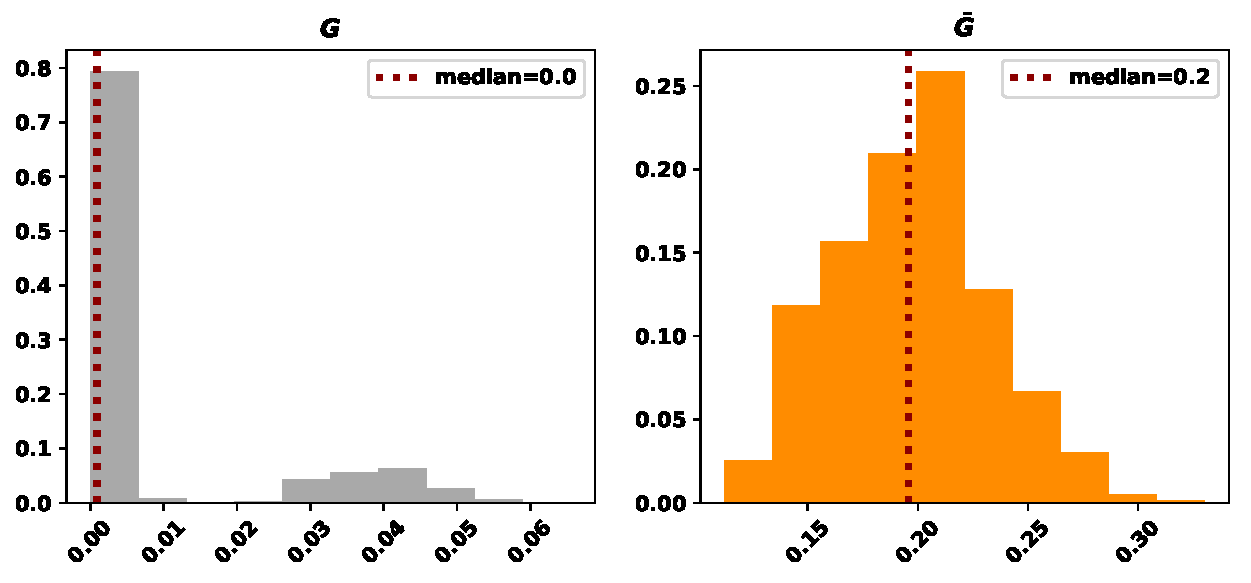
\includegraphics[width=.8\textwidth]{src/chapters/03/paper/bibliometric-study-of-the-prisoners-dilemma/assets/images/pd_closeness_centralities.pdf}
    \caption{Distributions of closeness centrality in \(G\) and \(\bar{G}\)}
    \label{fig:cc_distributions}
\end{figure}

\section{Distributions for topic networks}\label{appendix:distributions}

Betweeness and closeness centralities distributions for graphs of topics A to E.

\begin{figure}[!hbtp]
    \centering
    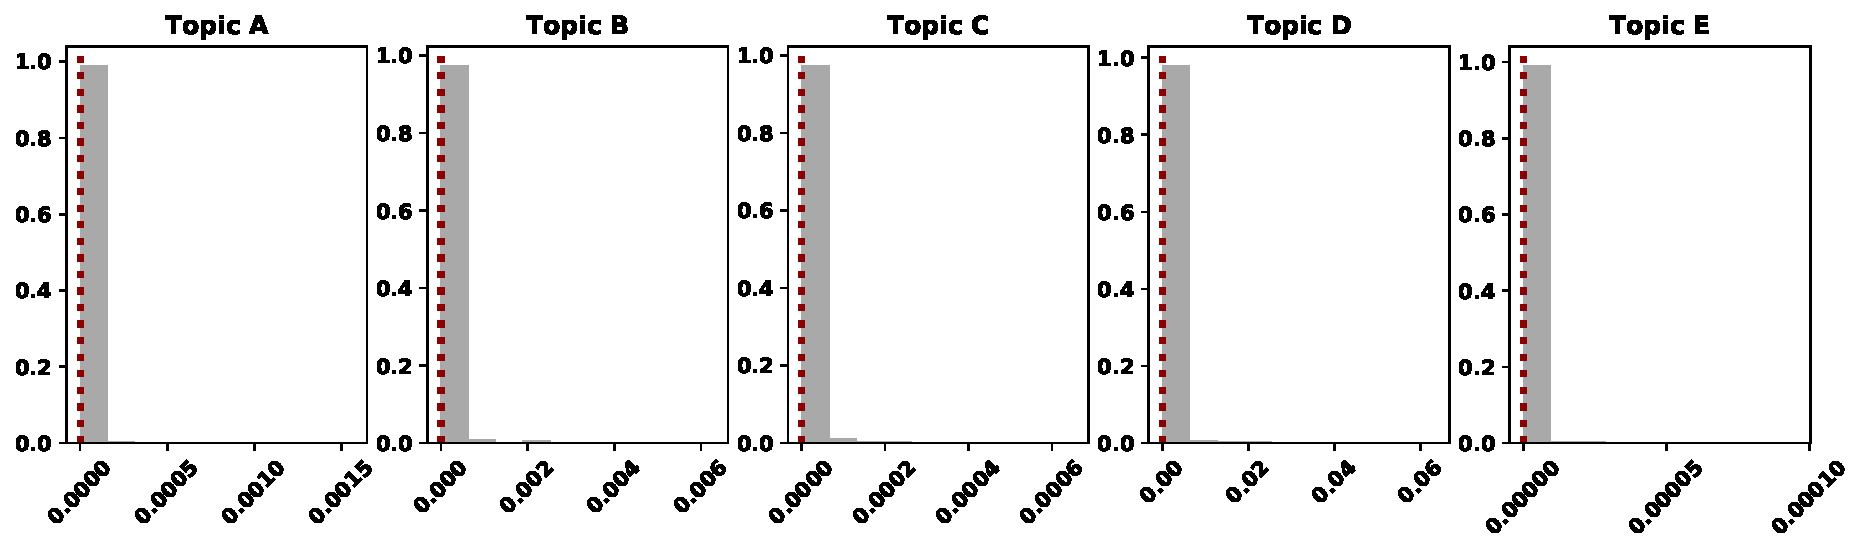
\includegraphics[width=\textwidth]{src/chapters/03/paper/bibliometric-study-of-the-prisoners-dilemma/assets/images/topics_betweeness_distributions.pdf}
    \caption{Distributions of betweenness centrality in topics' networks.}
    \label{fig:bc_distributions_topics}
\end{figure}

\begin{figure}[!hbtp]
    \centering
    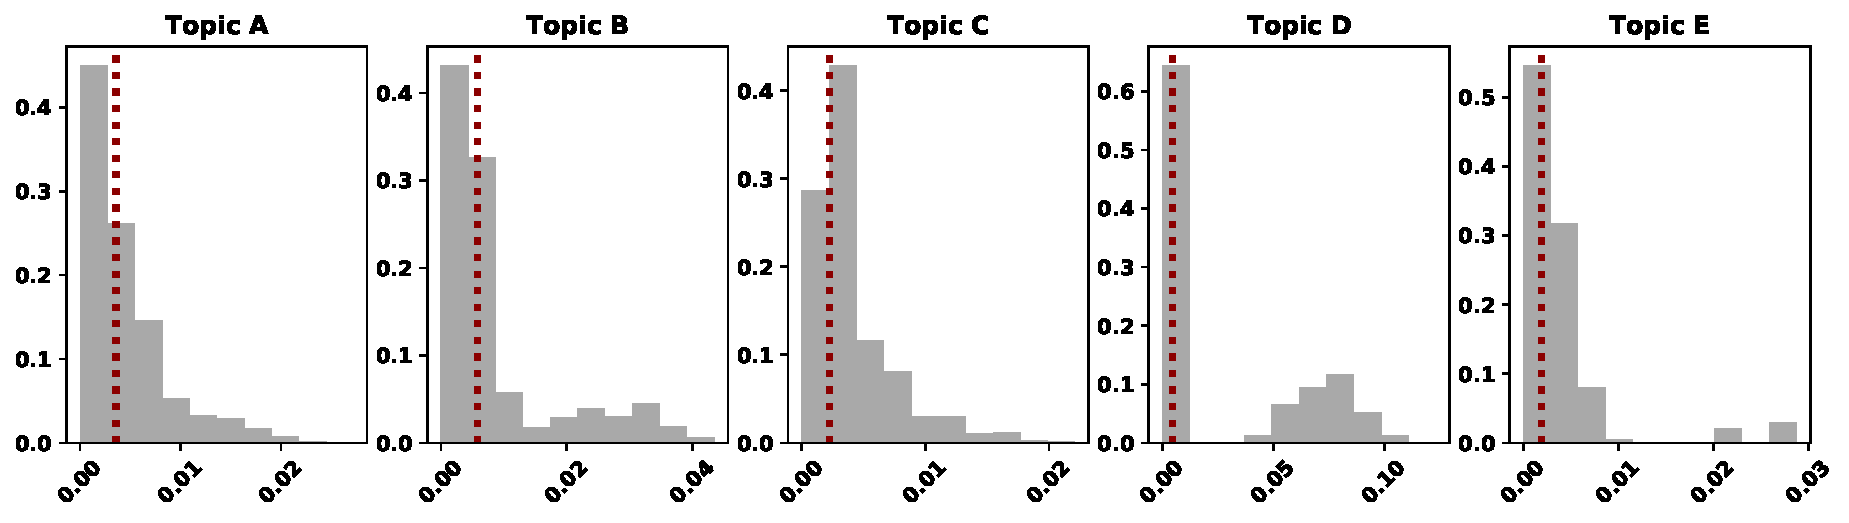
\includegraphics[width=\textwidth]{src/chapters/03/paper/bibliometric-study-of-the-prisoners-dilemma/assets/images/topics_closeness_distributions.pdf}
    \caption{Distributions of closeness centrality in topics' networks.}
    \label{fig:cc_distributions_topics}
\end{figure}
\end{appendices}

\end{document}
